\section{Literature Review}

Fabric classification has gained interest within computer vision and material science, with applications across many industries, including fashion, healthcare, manufacturing, and forensics. The advancements in deep learning have enabled researchers to develop automated approaches that accurately recognize and classify textile materials using image data. 

The traditional process of fabric classification has relied on manual methods and physical methods. Processes which are time-consuming, subjective to human error, and require equipment that could be specialized. The image-based classification of textiles and fabrics using deep learning models offers a more scalable and efficient approach and would allow for real-time implementations. 

In this section, we present key research contributions that have applied deep learning approaches to fabric classification because the datasets highlighted here (as used in these studies), are carefully considered when describing the research, as data quality and diversity are important when developing models that will be having a good performance. We also provide a detailed description of the three papers selected and implemented as part of this research work. Each paper takes a different modelling approach to highlight the merits and limitations of the current methodologies.

Through the exploration of all these work, we look to illuminate shared practices, inventive ideas, and existing issues in the domain, which have helped inform our proposed methodology.

\subsection{Dataset Overview}

The implementation and level of understanding of a strong, efficacious and generalized deep learning model that classifies fabrics is tied to the availability of high-quality, heterogeneous, and well-structured datasets. Each of the datasets provided in this domain provides textile properties from a fixed standpoint - with some focusing on fine surface-level textures, others providing microscopic or structural imaging, and others providing extensive predominately labeling through expert-based functional taxonomies.

Here, we provide our overview and review of three datasets which we utilized in the development and audit of our deep learning models for this research. These datasets were selected based upon relevance, heterogeneity, and the diversity of challenges that they represent in the fabric classification domain. Each dataset has helped inform our understanding of how fabrics presented visually, micro-structure, and material properties can be categorized in these helpful analyses. The datasets reviewed are described below:

\subsubsection{A. Fine-Grained Material Classification Using Micro-geometry and Reflectance~\cite{kampouris2016fine}}

One of the important base datasets for fine-grained material classification is based on detailed geometry and reflectance properties, introduced by Kampouris et al., which highlights slightly different materials through high-resolution images of shape, surface details, and reflections captured under different lighting conditions.

The dataset was captured using a custom-built photometric stereo sensor designed to acquire fine surface details of fabric materials. Each sample in the dataset corresponds to a small patch of fabric, captured under four different illumination conditions to facilitate the extraction of both micro-geometry (surface normals) and reflectance (albedo).

The dataset consists of several classes of fabrics that are listed in Table~\ref{tab:fabric_distribution}. Each class contains multiple samples, with each sample having four images corresponding to different light sources.

\begin{table}[H]
\centering
\caption{Fabric-wise Distribution of Samples and Images}
\label{tab:fabric_distribution}
\begin{tabular}{|l|c|c|}
\hline
\textbf{Fabric Class} & \textbf{Number of Samples} & \textbf{Total Images} \\
\hline
Acrylic & 12 & 48 \\
Artificial Fur & 1 & 4 \\
Artificial Leather & 3 & 12 \\
Blended & 411 & 1,644 \\
Chenille & 13 & 52 \\
Corduroy & 24 & 96 \\
Cotton & 588 & 2,352 \\
Crepe & 26 & 104 \\
Denim & 162 & 648 \\
Felt & 4 & 16 \\
Fleece & 33 & 132 \\
Leather & 16 & 64 \\
Linen & 19 & 76 \\
Lut & 4 & 16 \\
Nylon & 57 & 228 \\
Polyester & 226 & 904 \\
Satin & 24 & 96 \\
Silk & 50 & 200 \\
Suede & 5 & 20 \\
Terrycloth & 30 & 120 \\
Unclassified & 123 & 492 \\
Velvet & 11 & 44 \\
Viscose & 37 & 148 \\
Wool & 90 & 360 \\
\hline
\textbf{Total} & \textbf{2,048} & \textbf{8,192} \\
\hline
\end{tabular}
\end{table}


\begin{itemize}[noitemsep, topsep=0pt]
    \item \textbf{Images per sample:} 4 RGB images (one per light source)
    \item \textbf{Original resolution:} 640$\times$640 pixels
    \item \textbf{Cropped resolution:} 400$\times$400 pixels (to avoid out-of-focus regions)
    \item \textbf{Field of View:} Approximately 10 mm $\times$ 10 mm
    \item \textbf{Working Distance:} 3 cm - Distance from the camera to the fabric sample
\end{itemize}

\begin{figure}[H]
    \centering
    \begin{minipage}{0.8\linewidth}
        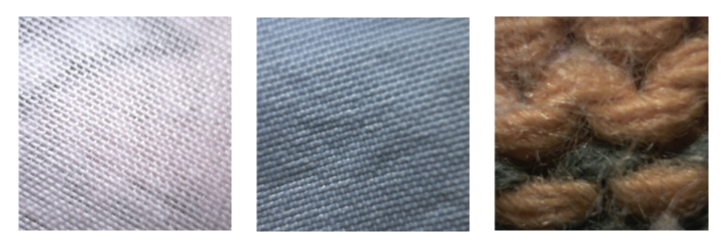
\includegraphics[width=\linewidth]{images/iBugDataset}
    \end{minipage}
    \caption[Sample images from the iBug Fabric Dataset]{Sample images from the iBug Fabric Dataset: (Left) Cotton, (Middle) Polyester, (Right) Wool.}
\end{figure}

\subsubsection{B. Optical Coherence Tomography Image Dataset of Textile Fabrics~\cite{sabuncu2022optical}}

The Optical Coherence Tomography (OCT) image dataset of textile fabrics is a distinct and specialized dataset comprised of high-resolution cross-sectional images of fabric structures. The dataset was produced by Sabuncu and Ozdemir, and thus far, has been used to support material classification tasks through depth imaging. Specifically, it has been helpful in textile engineering, recycling, and forensic investigations. 

The dataset includes OCT scans of fabrics made of only cotton, wool, and polyester. To accomplish this, three samples were taken from each of the three material types (cotton, wool, polyester) resulting in nine fabric types total. Each sample was scanned using the Thorlabs CAL110C1 OCT system over 100 random places on the surface of the sample with the objective of generating high-quality cross-sectional images or B-scans. The scans are all 2mm long and were excluded from other filtering options or pre-processing protocols, and were saved in raw \texttt{.png} images.

\begin{table}[H]
\centering
\caption{Class-wise image distribution of the Fabric OCT Dataset}
\begin{tabular}{|l|c|}
\hline
\textbf{Fabric Type} & \textbf{Number of images} \\
\hline
Cotton & 495 \\
Polyester & 448 \\
Wool & 533 \\
\hline
\end{tabular}
\end{table}

One of the main benefits of OCT imaging is that it shows aspects of a fabric’s internal microstructure that would be impossible to see from a standard RGB image: weave pattern, layer thickness, and material density internal to the fabric can provide great utility for classifying fabrics that may look the same on the surface. 

\begin{figure}[H]
    \centering
    \begin{minipage}{0.8\linewidth}
        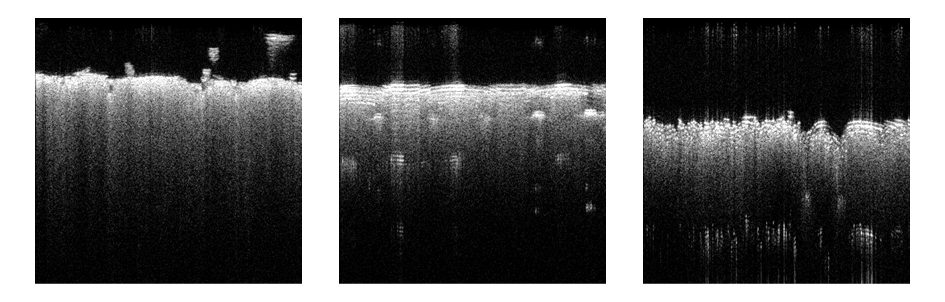
\includegraphics[width=\linewidth]{images/FabricOCTDataset.png}
    \end{minipage}
    \caption[Sample images from the Fabric OCT Dataset]{Sample images from the Fabric OCT Dataset: (Left) Cotton, (Middle) Polyester, (Right) Wool.}
\end{figure}

The dataset used in this project was organized into three folders, cotton, wool, and polyester, with multiple scans of different fabric pieces made from the same material per folder. A dataset organized this way is well-labeled and clean, supporting the training and testing of deep learning models, model architectures that will most likely learn from structural features rather than appearance. 

In summary, the OCT image dataset has a high degree of uniformity and detail, making it highly suitable for fine-grained classification of fabrics according to their internal structure. Additionally, its potential goes beyond classification, applications include recycling, identifying defects in textiles, and suitable for automated textile quality control assessments.

\subsubsection{C. TextileNet: A Material Taxonomy-Based Fashion Textile Dataset~\cite{zhong2023textilenet}}

TextileNet is a large-scale taxonomy-based dataset with the aim of facilitating textile material identification through deep learning methods. Originally proposed by Shu Zhong et al., TextileNet fills a significant gap that currently exists in datasets by providing a taxonomy of textile materials in a logical form covering two main branch of fibres and fabrics. In contrast to most datasets in the area of fashion that are poorly annotated and only provide mixed labels for fabric and fibre, or offer loose, ambiguous labels, TextileNet's labels are clearly defined with a scientific basis provided by material science researchers.

TextileNet consists of two datasets: \textit{TextileNet-fibre} and \textit{TextileNet-fabric}, with 33 fibre labels and 27 fabric labels included in the datasets. The combined dataset has approximately 760,949 images collected from Google Images and reconstituted fashion datasets such as iMaterialist. The images were collected based on keywords from subsequent queries which were derived from the defined textile taxonomy ensuring that the data collected conveys the type of real-world clothing items, but consistently added images in the same area across the project archive.

\begin{figure}[H]
    \centering
    \begin{minipage}{0.8\linewidth}
        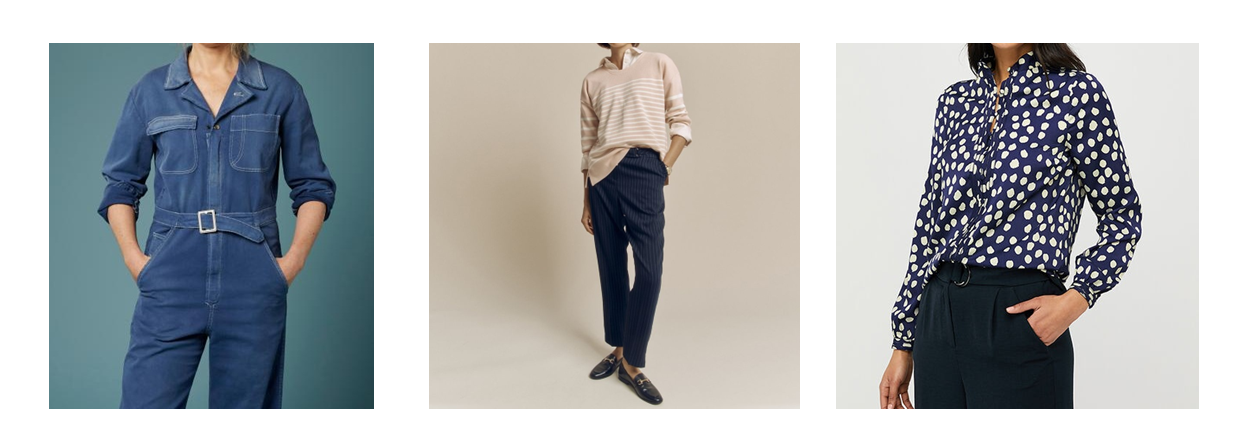
\includegraphics[width=\linewidth]{images/TextileNetDataset.png}
    \end{minipage}
    \caption[Sample images from the TextileNet Dataset]{Sample images from the TextileNet Dataset: (Left) Denim, (Middle) Crepe, (Right) Satin.}
\end{figure}

The value of TextileNet lies in its taxonomy-based structure. The fibre taxonomy range from natural, synthetic, and regenerated fibres (eg cotton, wool, polyester, bamboo viscose and milk casein). While the fabric taxonomy provides categories based on the methods of production (woven, knitted, non-woven), each with its examples (denim, tweed, velvet, jersey).

Overall, TextileNet is suitable for training efficient models for complex fabric composition recognition for both retail, recycling, supply chain application and as support to sustainable fashion design.

\subsection{Existing Work}

In recent years, deep learning has made incredible advancements in image-based classification tasks, including in textiles. There are several works that have explored Convolutional Neural Networks (CNNs) and vision transformer based architectures for classifying fabrics and textile compositions, achieving higher accuracy and robustness approaches. The incorporation of methods like transfer learning and dataset preparation can also assist the model's performance through lower accuracy losses, even when fabrics or textile compositions are not present in the original dataset, consisting of limited or domain specific images. 

This section is dedicated to reviewing a number of works that have been implemented where the results have been discussed as a component of this thesis. These papers show various methods for fabric classification, from a standard CNN to more advanced hybrid implementations utilising both Vision Transformers which develop capabilities to quickly compose hybrid pipelines with conventional statistical techniques literature including Principal Component Analysis (PCA) and Linear Discriminant Analysis (LDA).

Each implemented study communicated various solutions to fabric classification issues and approaches. By executing and discussing each of the works, there will be further understanding for any potential challenges with classification of textile data using various deep learning models. The study results will also allow the collective and reasoning to create a more effective and efficient hybrid model.

\subsubsection[A. Research on Classification of Clothing Fabrics Images Based on Convolutional Neural Network]{A. Research on Classification of Clothing Fabrics Images Based on Convolutional Neural Network~\cite{hong2024research}}

In the paper \textit{"Research on Classification of Clothing Fabrics Images Based on Convolutional Neural Network"} by Ying Hong and others the authors take use of a machine learning construct to identify clothing fabric types from image data automatically. The authors understand that there is an increasing need for intelligent systems related to fabric identification, since fabric identification in clothing design and fabric production is often a manual process which can be time-consuming and inconsistent.

The authors utilize a transfer learning approach by fine-tuning the VGG-16 model, which is a pre-trained convolutional neural network architecture on the ImageNet dataset, to meet the study demands. An important note here is that the study uses a custom dataset which includes 15,000 images of previously unseen, high-quality images of 10 different types of clothing fabrics (cotton, wool, silk, denim, etc.). The images were taken in a controlled lighting environment as this was useful to keep lighting consistent as possible and reduce noise from the background.

\begin{figure}[H]
    \centering
    \begin{minipage}{1\linewidth}
        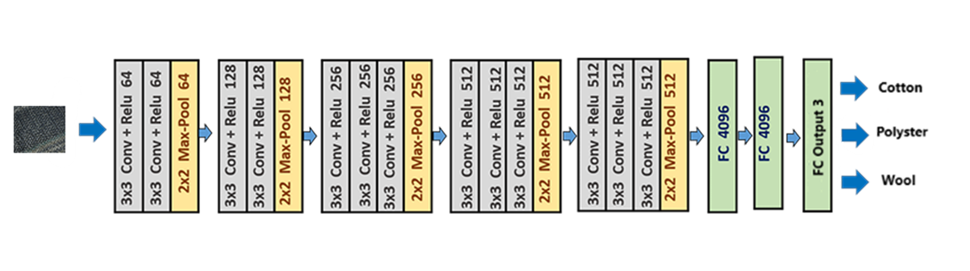
\includegraphics[width=\linewidth]{images/Paper1Model.png}
    \end{minipage}
    \caption[Model architecture - Hong et al.~\cite{hong2024research}]{Model architecture used for classification in Hong et al.~\cite{hong2024research}.}
\end{figure}

Data augmentation is also implemented in this study to improve model generalization. Data augmentations included object rotation, flipping, brightness adjustment, and adding Gaussian noise. Data augmentations will force the network to learn invariant features to some extent and involved overfitting.

The model was able to achieve the test accuracy of 99.73\% and also achieved a significant level of performance in differentiating between fabrics that visually appeared the same. The authors pointed out the fast convergence capability and robust classification ability of the proposed model, as well as the proposed convolutional networks, could possibly be applied to problems of practical importance in the clothing and fabric industry, even architectures with moderate depth like VGG-16.

This study demonstrates the advantages of incorporating transfer learning with well-curated datasets and simple preprocessing steps. It reaffirms the suitability of CNN-based approaches for fabric classification, particularly for high-quality image data. Furthermore, this study creates an opportunity for future work to explore advanced architectures or, for multi-modal data sources.

\subsubsection[B. TextileNet: A Deep Learning Approach for Textile Fabric Material Identification from OCT and Macro Images]{B. TextileNet: A Deep Learning Approach for Textile Fabric Material Identification from OCT and Macro Images~\cite{siam2023textilenet}}

In Siam et al.'s paper \textit{"TextileNet: A Deep Learning Approach for Textile Fabric Material Identification from OCT and Macro Images"}, the authors explore the efficiency of deep learning models for automatic classification of fabric material types based upon macro images and Optical Coherence Tomography (OCT) images. This study is creating a solution for recognizing the class features of fabrics like cotton, wool, and polyester, all of which present very similar visual appearances to the human eye but have different structure, property, and resilience.

\begin{figure}[H]
    \centering
    \begin{minipage}{1\linewidth}
        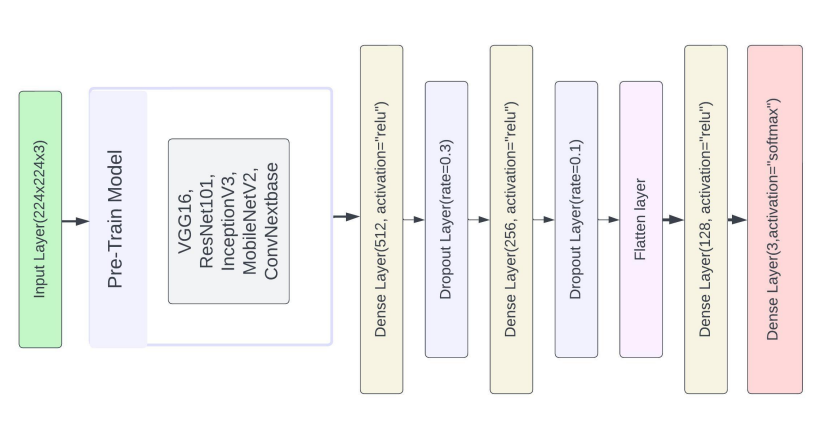
\includegraphics[width=\linewidth]{images/Paper2Model.png}
    \end{minipage}
    \caption[Model architecture - Siam et al.~\cite{siam2023textilenet}]{Model architecture used for fabric classification in Siam et al.~\cite{siam2023textilenet}}
\end{figure}

This article presents a deep learning classification pipeline model based on transfer learning. The authors employed five different deep-learning convolutional neural networks: MobileNetV2, VGG16, ResNet101, InceptionV3, and ConvNextBase. The authors adapted and fine-tuned the five networks to classify textile sample types based on visual feature and structure.

The authors also applied image processing techniques for improved image quality and model performance, which included grayscale, contrast limiting adaptive histogram equalization (CLAHE), and sharpening effect. All images were also resized to the standard image input size size of 224 pixels high and 224 pixels wide.

The results indicate that MobileNetV2 outperformed all the models by a wide margin, with 99.87\% accuracy on OCT images and 95.17\% accuracy on macro images. The performance gap between the two was significant; this indicates the additional value of utilizing OCT imaging for the discrimination of fabrics as it provided insight into deep structural features that were not revealed with a surface-based macro image.

This work shows that deep learning coupled with high-resolution image modalities such as OCT can offer not only a reliable but highly accurate soft fabric classification. Considering that the proposed bio-inspired pipeline is lightweight and efficient, it can be easily implemented in a multitude of real-world applications in the textile industry such as automated material sorting, automated quality control, and textile recycling.

\subsubsection[C. Fabric Composition Identification using Fine-Tuned Vision Transformers]{C. Fabric Composition Identification using Fine-Tuned Vision Transformers~\cite{chitra2023fabric}}

The current study \textit{"Fabric Composition Identification using Fine-Tuned Vision Transformers"} by Chitra G M et al. shows an innovative and modern technique to classify fabric using Vision Transformers (ViTs) instead of solely relying on convolutional features as explored in the literature. This work captures and understands feature representations at both local and global scales via transformer based architectures for fabric images. Our main objective in this study is to identify fabric compositions given fabrics could take on a blend with multiple fibres as input. 

In the dataset, 937 images were collected and labelled as multiple types of fabrics: cotton, polyester, nylon, silk etc. These images were captured using smartphone cameras, to represent realistic circumstances where users or retailers might classify fabric type using their frequently employed devices. The practical nature of this setup allows for the proposed approach to be used for a mobile or on-site fabric classification application.

The pipeline proposed comprises several steps; image features are first extracted from a fine-tuned ViT model. Features are then reduced with Principal Component Analysis (PCA), then subsequently, Linear Discriminant Analysis (LDA), which was applied later to reduce the features in order to enhance class separation before applying the classifier, Support Vector Machine (SVM). Furthermore, the authors applied Platt scaling on the SVM to gain an understanding of predicted probability outputs and associated confidence.

\begin{figure}[H]
    \centering
    \begin{minipage}{1\linewidth}
        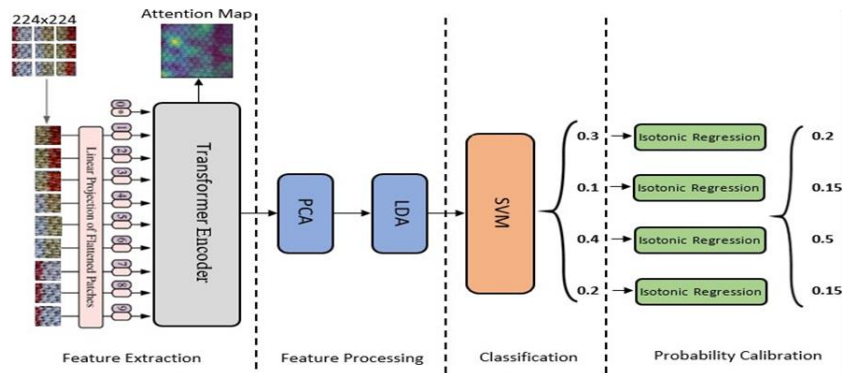
\includegraphics[width=\linewidth]{images/Paper3Model.png}
    \end{minipage}
    \caption[Model architecture - Chitra G M et al.~\cite{chitra2023fabric}]{Model architecture used for fabric composition identification in Chitra G M et al.~\cite{chitra2023fabric}}
\end{figure}

The model has an average F1-score of 0.87, a mean squared error (MSE) value of 0.20, and log-loss of 0.44. These results show that the pipeline is effective in reliably identifing pure and mixed fabric types from images. Moreover, the authors use SHAP (SHapley Additive exPlanations) values to add further interpretability to the model, indicating the parts of the image that influenced the classification decision. This could be especially well suited to help understand where the model may be differentiating blended materials. 

In summary, this work demonstrates the potential of Vision Transformers for fabric composition evaluation. The hybrid method of combining ViTs with more conventional dimensionality reduction and machine learning classifiers can practically be implemented in practical settings in application situations ranging from quality control, textile recycling, and remote rugged garment identification.
